\documentclass{article}

\usepackage{url,graphicx,tabularx,array,geometry, hyperref}
\usepackage{listings}
\usepackage{fullpage}
\usepackage{fancyvrb}
\usepackage{framed}
\usepackage{lastpage}
\usepackage{fancyhdr}

\renewcommand{\headrulewidth}{0pt}
\setcounter{secnumdepth}{0}

\setlength{\parskip}{1ex} %--skip lines between paragraphs
\setlength{\parindent}{0pt} %--don't indent paragraphs
\setlength{\headheight}{15.2pt}

\pagestyle{fancy}

\renewcommand{\headrulewidth}{0pt}
\lhead{  }
\lfoot{Lab 1: TCP Congestion Control}
\rfoot{page \thepage\ of \pageref{LastPage}}

\renewcommand{\familydefault}{\sfdefault}
\begin{document}

\begin{titlepage}
\begin{center}
\textsc{\huge \bfseries Advanced Networking 2018}\\[1.5cm]
\textsc{\large Lab \#1: TCP Congestion Control}\\[1.5cm]
\textsc{\huge Report}\\[1.5cm]
\textsc{\huge \bfseries GROUP: 1}\\[1.5cm]
\textsc{\large{\textbf{Authors:}\\ Rick van Gorp, rick.vangorp@os3.nl\\ Luc Gommans, os3@lucgommans.nl}}

\textsc{\large University of Amsterdam}
\end{center}
\end{titlepage}

\subsection{Q1.1 Plot a graph showing CWND versus time from 0.0s to 100.0s.}

\begin{figure}[H]
	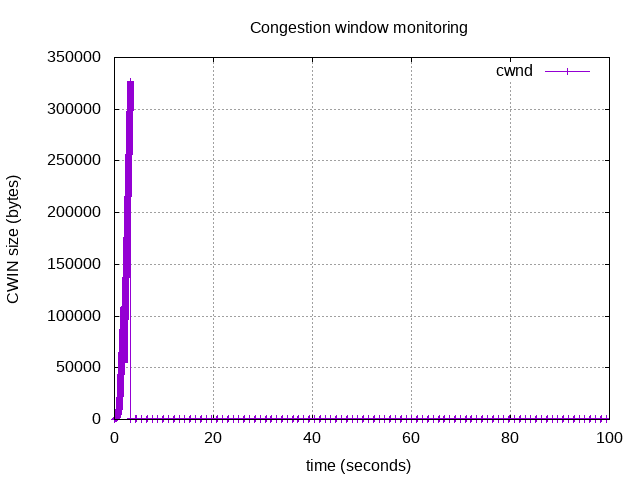
\includegraphics{lab1-group1-task1-question1.png}
	%\label{fig:dinges}
	\caption{T1Q1 CWND from 0 to 100 seconds}
\end{figure}


\subsection{Q1.2 Plot a graph showing SSTH versus time from 0.0s to 100.0s.}

\begin{figure}[H]
	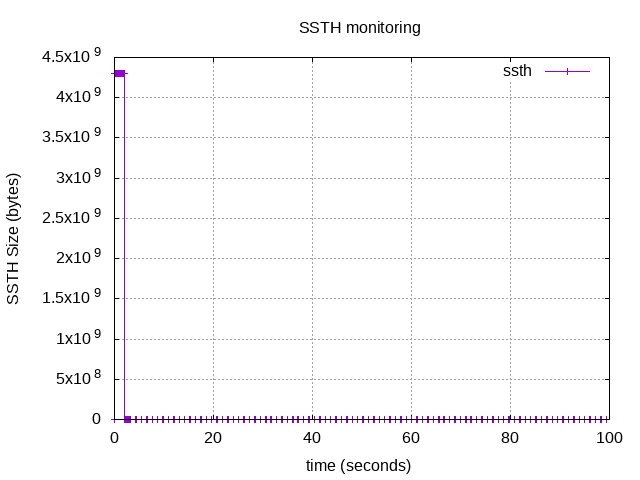
\includegraphics{lab1-group1-task1-question2.png}
	%\label{fig:dinges}
	\caption{T1Q2 SSTH from 0 to 100 seconds}
\end{figure}


\subsection{Q1.3 Find the points where the slow-start, congestion-avoidance, fast retransmit/fast recovery states begin.}

TODO

\begin{table}[H]
\begin{tabular}{|c|p{25mm}|p{20mm}|c|c|}
\hline Time (s)    & Current CWND (bytes)    & New CWND (bytes)    & New State             & Event            \\
\hline 0.00000     & 0                       & 340                 & slow-start            & start            \\ 
\hline 1.93189     & 109 480                 & 55 590              & fast-recovery         & dupACKcount==3   \\ 
\hline 3.26916     & 326 570                 & 340                 & slow-start            & timeout          \\ 
\hline 3.30286     & 340                     & 680                 & congestion-avoidance  & cwnd$>=$ssthtresh  \\ 
\hline  
\end{tabular} 
\end{table}


\subsection{Q1.4 Plot a graph showing CWND versus time from 0.0s to 100.0s.}

\begin{figure}[H]
	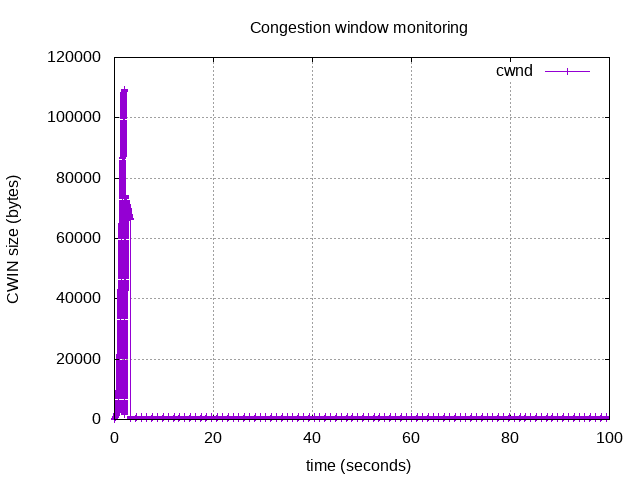
\includegraphics{lab1-group1-task1-question4.png}
	%\label{fig:dinges}
\end{figure}


\subsection{Q1.5 Plot a graph showing SSTH versus time from 0.0s to 100.0s.}

\begin{figure}[H]
	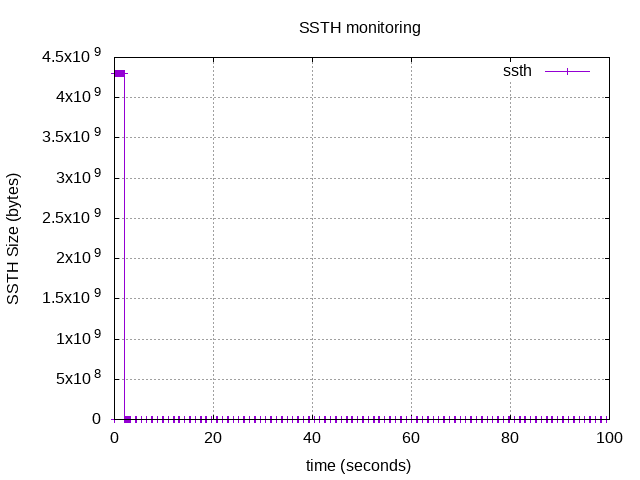
\includegraphics{lab1-group1-task1-question5.png}
	%\label{fig:dinges}
\end{figure}


\subsection{Q1.6 Find the points where the slow-start, congestion-avoidance, fast retransmit/fast recovery states begin.}

TODO

\begin{table}[H]
\begin{tabular}{|c|p{25mm}|p{20mm}|c|c|}
\hline Time (s)    & Current CWND (bytes)    & New CWND (bytes)    & New State             & Event            \\
\hline 0.00000     & 0                       & 340                 & slow-start            & start            \\ 
\hline 1.21176     & 163 882                 & 82 790              & fast-recovery         & dupACKcount==3   \\ 
\hline ???????     & 326 570                 & 340                 & slow-start            & timeout          \\ 
\hline 2.54903     & 151 810                 & 340                 & fast-recovery         & TODO \\ 
\hline  
\end{tabular} 
\end{table}


\subsection{Q1.7 Discuss and motivate the differences you observe between the NewReno and this algorithm.}

TODO

\subsection{Q2.1 Plot a graph showing the CWND and ssthresh versus time with all the data you get. These two metrics are in one graph.}

\begin{figure}[H]
	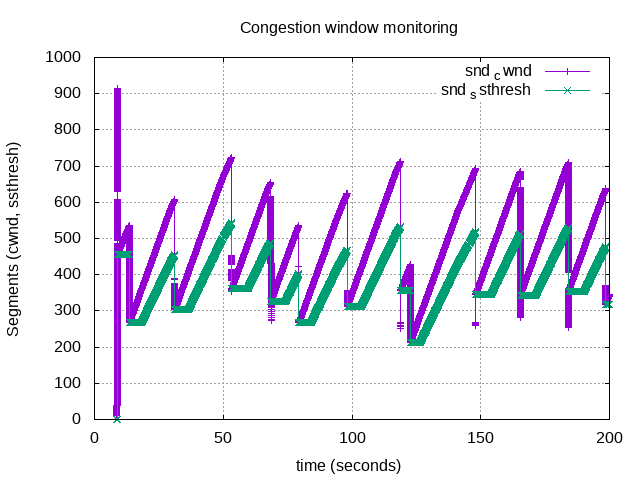
\includegraphics{lab1-group1-task2-question1.png}
	%\label{fig:dinges}
\end{figure}


\subsection{Q2.2 Briefly discuss the changing process.}

\subsection{Q2.3 Plot a graph showing CWND versus time with all the data you get.}

\begin{figure}[H]
	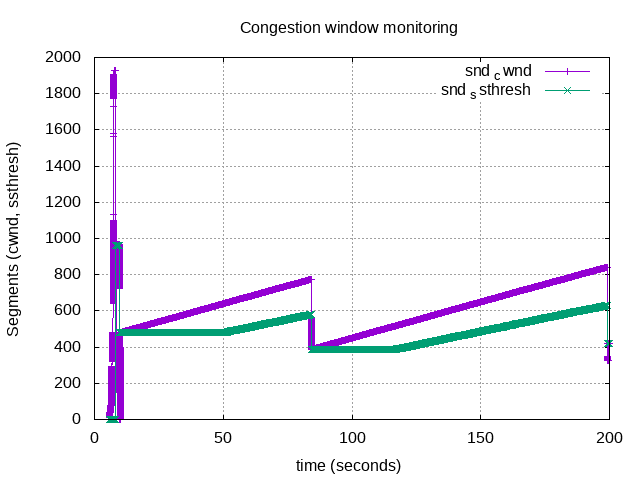
\includegraphics{lab1-group1-task2-question3.png}
	%\label{fig:dinges}
\end{figure}


\subsection{Q2.4 Compare this graph with the one from}

\subsection{Q2.5 Plot a graph showing CWND and ssthresh versus time with all the data you get.}

\subsection{Q2.6 Compare this graph with the graph of}

\subsection{Q2.7 Zoom in the graph of this scenario (plot some parts of this scenario in a short duration, 10 or 20 seconds). Briefly explain the changing process.}

\subsection{Q2.8 Show a screen capture of the real throughput in this scenario.}

\subsection{Q2.9 Plot a graph showing CWND and ssthresh versus time with all the data you get.}

\subsection{Q2.10 Compare this graph with the graph of}

\subsection{Q2.11 Plot a graph showing CWND and ssthresh versus time with all the data you get.}

\subsection{Q2.12 Compare this graph with the graph of scenario three and show the differences.}

\subsection{Q2.13 Zoom in the graph of this scenario (plot some parts of this scenario in a short duration, 10 or 20 seconds). Briefly explain the changing process and compare it with the graph of}

\subsection{Q2.14 Show a screen capture of the real throughput and compare it with throughput of}

\subsection{Q3.1 Explain what an LFN network is. Change the simulation parameters to your likings and demonstrate that TcpNewReno is not suitable for LFN networks.}

\subsection{Q3.2 Explain SACK does. Change the simulation parameters to your likings and demonstrate the performance improvement with SACK.}

\subsection{Q3.3 Explain with TCP fairness is. Show the effect of multiple flows in the simulation.}

\subsection{Q3.4 Replicate scenario 3 of the emulation: packet loss of 3\%, delay of 50 ms and transfer duration of 200sec. Use TcpNewReno. Compare the two results.}

\subsection{Q3.5 After these experiments, please briefly describe the difference between simulation and emulation?}

\end{document}
